\documentclass[conference]{IEEEtran}
\IEEEoverridecommandlockouts

\usepackage[T1]{fontenc}
\usepackage[utf8]{inputenc}
\usepackage{cite}
\usepackage{amsmath,amssymb}
\usepackage[scaled=0.83]{beramono}
\usepackage{booktabs}
\usepackage{tabularx}
\usepackage{array}
\usepackage{tikz}
\usetikzlibrary{arrows.meta,positioning,calc}
\usepackage[hyphens]{url}
\usepackage[hidelinks]{hyperref}
\hypersetup{
  pdftitle={svcc: Translation-Validated Bidirectional Compilation Between SystemVerilog/UVM and C++17 SystemC},
  pdfauthor={Mayur Kubavat},
  pdfkeywords={ASIC verification, SystemVerilog, UVM, SystemC, CRAVE, FC4SC, translation validation, sequential equivalence checking}
}
\usepackage{orcidlink}
\usepackage{microtype}

\Urlmuskip=0mu plus 1.5mu\relax
\setlength{\emergencystretch}{1.4em}
\newcommand{\code}[1]{{\fontshape{n}\ttfamily #1}}

\pagestyle{plain}

\begin{document}

\title{svcc: Translation-Validated Bidirectional Compilation Between SystemVerilog/UVM and C++17 SystemC\thanks{This work was done independently, on personal equipment and in a personal capacity. It is not affiliated with or endorsed by any employer.}}

\author{\IEEEauthorblockN{Mayur Kubavat\,\orcidlink{0009-0009-1087-8558}}
\IEEEauthorblockA{\textit{Independent Researcher, Mountain View, CA, USA}}}

\maketitle
\thispagestyle{plain}

\begin{abstract}
In ASIC verification, teams often write fast reference models and license-free testbenches in C++17 and IEEE~1666-2023 SystemC, while RTL sign-off and coverage closure still run in IEEE~1800-2023 SystemVerilog, IEEE~1800.2-2020 UVM, and SystemVerilog Assertions (SVA). Translating code across these two stacks by hand or with an unverified language model introduces quiet bugs. Garbage-collected UVM handles clash with value-copied C++ transaction ports, SystemVerilog context-determined bit widths differ from C++ integer promotion, Preponed \code{\#1step} sampling races against SystemC delta notifications, and large CRAVE constraint blocks trigger superlinear C++ template compile times.

This paper presents \code{svcc}, an open-source Rust compiler and translation-validation tool (12,600 lines of Rust across eight crates plus Python bindings) that translates in both directions between SystemVerilog (RTL and UVM testbench components) and C++17 SystemC~3.0.3 (IEEE~1666.1 RTL, UVM-SystemC, CRAVE, FC4SC, and untimed C++17 reference functions). Both languages lower into a typed seven-dialect intermediate representation (\code{svcc-ir}). Target-specific passes legalize each direction, including hard-bound clipping and least-common-multiple (LCM) scaling for \code{dist} ranges, per-age hit counters for \code{cover property}, and a 32-bit cycle-walking Feistel generator for \code{randc}. Every run can be checked without a commercial simulator by four solver gates: a Z3 \code{QF\_BV} miter over constraints, enums, and \code{dist} support; bounded model checking (BMC) of generated C++17 SVA observers; UCIS~1.0 coverage bin isomorphism; and word-level Btor2 sequential equivalence checking (SEC) across pipeline latency $L \ge 0$. On a 20-design benchmark suite, \code{svcc} translates files in 272~$\mu$s median (\code{sv2sc}) and 689~$\mu$s median (\code{sc2sv}, with \code{svlang-lint}), proves all 20 round-trip and all 8 C-to-RTL checks in 5.37--21.68~ms, catches 20 of 20 injected bugs with 0 false alarms on 4 equivalent rewrites, and recovers 12 of 12 standalone UVM/RAL files without package filelists (against 4 of 12 for semantic-only lowering). Splitting CRAVE clauses cuts \code{clang++ -O2} compile time at 120 clauses by $6.25\times$. Against live Accellera libraries, \code{svcc} cuts sliced-\code{dist} sampling error by $60.8\times$, speeds up 10-bit \code{randc} solving by $341\times$, and lowers 9 of 12 unmodified files from OpenTitan, PULP, OpenHW, and Ibex.
\end{abstract}

\begin{IEEEkeywords}
ASIC verification, SystemVerilog, SystemC, UVM, translation validation, constrained-random verification, sequential equivalence checking.
\end{IEEEkeywords}

\section{Introduction}
\label{sec:intro}

Hardware teams frequently keep two versions of the same block or testbench component, one in C++ and one in SystemVerilog. Cycle-fast predictors, software-driven stimulus, and Verilator harnesses~\cite{snyder2020verilator} use C++17 and IEEE~1666-2023 SystemC~\cite{ieee1666_2023,ghenassia2005tlm} together with the open Accellera verification libraries: UVM-SystemC, CRAVE~\cite{haedicke2012crave}, and FC4SC~\cite{accellera2026systemc}. Tape-out sign-off, assertion checking, and functional coverage closure still depend on IEEE~1800-2023 SystemVerilog~\cite{ieee1800_2023} and IEEE~1800.2-2020 UVM~\cite{ieee1800_2_2020}. Recent benchmarks on RTL generation~\cite{liu2023verilogeval,thakur2024verigen} and SystemC library maintenance~\cite{kubavat2026scbench} show why both stacks stay in daily use. A single C++ testbench rebuilds and runs in about a second without waiting on simulator licenses, while final block sign-off expects native SystemVerilog assertions, covergroups, and register models.

Keeping parallel SystemVerilog and C++ sources aligned by hand is tedious and error-prone. Current open-source tools cover one direction or one layer of the stack. Verilator~\cite{snyder2020verilator} compiles SystemVerilog RTL into fast C++ simulation models, not readable UVM-SystemC classes or CRAVE constraints, and does not translate C++ back to SystemVerilog. Synthesis and compiler frameworks such as Yosys~\cite{wolf2013yosys}, LLHD~\cite{schuiki2020llhd}, and CIRCT~\cite{lattner2021mlir,circt2024} handle netlists and behavioral RTL, leaving out \code{rand}/\code{randc} constraints, weighted \code{dist} clauses, covergroup crosses, UVM register abstraction layer (RAL) maps, and \code{fork}/\code{join\_any}/\code{disable fork} blocks. Asking a language model to rewrite a SystemVerilog sequence item or RTL block into C++ produces code that often compiles, yet silently changes bit widths, signedness, or constraint rules.

In verification, a design or model is not trusted because it looks plausible. It is trusted because it passed an explicit sign-off check. This paper applies translation validation~\cite{pnueli1998tv,lopes2021alive2} to bidirectional SystemVerilog and SystemC compilation. Instead of assuming the translator has no bugs, \code{svcc} checks every output with host compilers (\code{clang++ -Werror}, \code{svlang}, and \code{svlang-lint}~\cite{kubavat2026svlang}) and proves equivalence across constraints, assertions, covergroups, and clocked RTL using Z3~\cite{demoura2008z3} and Btor2~\cite{niemetz2018btor2}.

This paper makes four contributions:
\begin{enumerate}
\item \textbf{A seven-dialect intermediate representation (\code{svcc-ir}).} A typed Rust IR models bit-accurate types, UVM classes and RAL maps, arena-indexed random constraints, UCIS~1.0~\cite{accellera_ucis10} covergroups, phase and clocking schedules, concurrent SVA properties, and synthesizable RTL processes (Sections~\ref{sec:impedance} and~\ref{sec:arch}).
\item \textbf{Hybrid semantic/CST lowering and solver-aware C++17 emission.} \code{svcc-front-sv} combines \code{svlang} elaboration and \code{TypeOracle} constant folding with concrete syntax tree (CST) fallback so single UVM files translate without full \code{uvm\_pkg} filelists. \code{svcc-emit-sc} splits large CRAVE constraints to avoid Boost.Proto compile-time blowup~\cite{veldhuizen1995expr}, clips and LCM-scales \code{dist} \code{:/} ranges, and emits a 32-bit cycle-walking Feistel \code{randc} generator (Section~\ref{sec:arch}).
\item \textbf{Four solver-backed checks and C-to-RTL equivalence.} \code{svcc-equiv} proves constraint equivalence in \code{QF\_BV}, checks 64-bit shift-window \code{assert property} observers and per-age \code{cover property} counters by bounded model checking, verifies UCIS~1.0 bin isomorphism, and lowers untimed C++17 functions (\code{// svcc:c2rtl}) into static single assignment (SSA) cones checked against pipelined RTL across latency $L \ge 0$ (Section~\ref{sec:equiv}).
\item \textbf{Measurements on synthetic, live-library, and external silicon code.} I evaluate \code{svcc} across 20 benchmark designs, 24 mutation and equivalent-rewrite checks, standalone VIP and clause-count ablations, live SystemC/UVM-SystemC/CRAVE/FC4SC execution, $10^7$-cycle SVA runs, and 12 unmodified files from OpenTitan, PULP, OpenHW, and lowRISC Ibex (Section~\ref{sec:eval}).
\end{enumerate}

\section{Where SystemVerilog and SystemC Diverge}
\label{sec:impedance}

\begin{table*}[t]
\centering
\caption{Seven language mismatches between IEEE 1800-2023 SystemVerilog/UVM and C++17 SystemC 3.0.3 handled by \code{svcc}.}
\label{tab:impedance}
\footnotesize
\begin{tabularx}{\textwidth}{@{}>{\raggedright\arraybackslash}p{1.00in} >{\raggedright\arraybackslash}p{1.52in} >{\raggedright\arraybackslash}p{1.52in} >{\raggedright\arraybackslash}X@{}}
\toprule
\textbf{Area} & \textbf{SystemVerilog / UVM} & \textbf{C++17 SystemC / CRAVE} & \textbf{\code{svcc-ir} Pass \& Sign-Off Check} \\
\midrule
Object \& TLM copy & Garbage-collected handles; \code{`uvm\_field\_int} flags & Value-copied \code{tlm\_analysis\_port}; \code{crv\_variable<T>} solver refs & \code{OwnershipPass} generates copy ctors and \code{do\_copy} that copy scalar values without corrupting solver node IDs. \\
Bitvector arithmetic & Context-determined width; unsigned turns signed math unsigned & C++ integral promotion (\code{uint8\_t + uint8\_t -> int}) & \code{WidthSignednessPass} records $(W, s)$ on every node; Z3 \code{QF\_BV} miter checks exact sign and zero extension. \\
CRV tolerances, \code{dist} \& \code{randc} & \code{inside \{[c +/- d], [c +\%- p]\}}, \code{:=}/\code{:/} weights, 32-bit \code{randc} & \code{crave::dist}, \code{weighted\_range}, 16-bit \code{randc} limit & Expands tolerances, clips \code{:/} ranges to hard bounds + $u128$ LCM, emits \code{svcc\_randc\_feistel<W>}, and checks support in Z3. \\
Process cancellation & \code{fork ... join\_any; disable fork;} kills sibling threads & \code{sc\_spawn} threads have no safe stack-unwinding \code{kill()} & \code{sched} dialect emits an \code{sc\_event\_or\_list} barrier and a shared \code{std::atomic<bool>} cancel token. \\
Clocking skew & \code{clocking cb @(posedge clk); input \#1step} (Preponed) & \code{posedge\_event()} wakes in the evaluate/delta phase & Emits an \code{svcc\_clocking\_*} snapshot struct sampled from the SystemC~3.0.3 \code{SC\_PRE\_TIMESTEP} callback. \\
Pipelined SVA & Concurrent \code{ant |-> \#\#[m:n] con} (\code{assert} \& \code{cover}) & No built-in temporal assertion engine in IEEE~1666 & Emits \code{uint64\_t pending\_window\_} (\code{assert}) and \code{pending\_age\_} (\code{cover}); Z3 BMC proves cycle and hit-count parity. \\
RTL \& C2RTL & \code{always\_comb}, \code{always\_ff}, nonblocking \code{<=} & \code{SC\_METHOD}/\code{SC\_CTHREAD} or untimed C++17 functions & Refuses heap/recursion fail-closed per IEEE~1666.1~\cite{ieee1666_1_2016}; unrolls bounded loops and branches to SSA muxes for Btor2 SEC. \\
\bottomrule
\end{tabularx}
\end{table*}

Line-by-line syntax translation between SystemVerilog and C++17 breaks down on everyday testbench and RTL idioms. Table~\ref{tab:impedance} lists seven places where the two languages assign different meanings to similar code, along with how \code{svcc} handles each case.

The first mismatch is object copying across TLM ports. In UVM-SystemC, \code{uvm::\allowbreak uvm\_\allowbreak analysis\_\allowbreak port<T>} passes sequence items by C++ value or reference, while each CRAVE random variable (\code{crave::\allowbreak crv\_\allowbreak variable<T>}) registers an internal solver node ID inside its parent \code{crave::\allowbreak rand\_obj}~\cite{haedicke2012crave}. A default C++ copy constructor copies that solver handle instead of just the randomized value, which breaks later \code{randomize()} calls and scoreboard comparisons. \code{OwnershipPass} detects classes with random fields and marks them for custom copy constructors, \code{do\_copy}, \code{do\_print}, \code{do\_pack}, \code{do\_unpack}, and \code{do\_compare} methods that respect \code{UVM\_NOCOMPARE} and \code{UVM\_NOCOPY}. Derived UVM sequence-item constructors also pass \code{crave::\allowbreak crv\_\allowbreak object\_\allowbreak name} by value so CRAVE's internal hierarchy stack is not popped before member constraints register.

The second mismatch is bit-width and sign propagation. SystemVerilog sizes arithmetic from the surrounding context and makes an expression unsigned if any operand is unsigned. C++ instead promotes narrow unsigned types (\code{uint8\_t}, \code{uint16\_t}) to signed 32-bit \code{int}. \code{svcc-ir} stores explicit bit width and signedness on every constant and variable so the emitters and the Z3 \code{QF\_BV} encoder apply the same extension and masking rules.

The third mismatch is overlapping pipelined assertions. A concurrent property \code{ant |-> \#\#[m:n] con} starts a fresh check on every clock edge where \code{ant} holds, even while earlier transactions are still in flight. A naive C++ translation using one counter drops overlapping bursts. For windows $0 \le m \le n < 64$, \code{svcc-emit-sc} lowers \code{assert property} into a constant-time 64-bit shift register (\code{pending\_window\_ = (pending\_window\_ <\kern0pt< 1) | ant}). Because one bit per age merges simultaneous threads when counting cover hits, \code{cover property} lowers to a per-age counter array (\code{pending\_age\_}) so burst hit counts match IEEE~1800.

The fourth mismatch is untimed C++ reference code versus clocked RTL. C++ predictors update local variables imperatively across \code{if}/\code{else} branches and bounded loops, while RTL spreads the same logic across pipeline stages. Following word-level C-to-RTL checking~\cite{koelbl2009c2rtl}, \code{svcc} restricts \code{C2RTL} inputs to the IEEE~1666.1 synthesizable subset~\cite{ieee1666_1_2016}. It rejects pointers, heap containers, floating-point types, and unbounded loops fail-closed, then turns sequential variable writes into SSA mux trees checked against the RTL module at latency $L$.

\section{Architecture and the svcc-ir Representation}
\label{sec:arch}

\begin{figure*}[t]
\centering
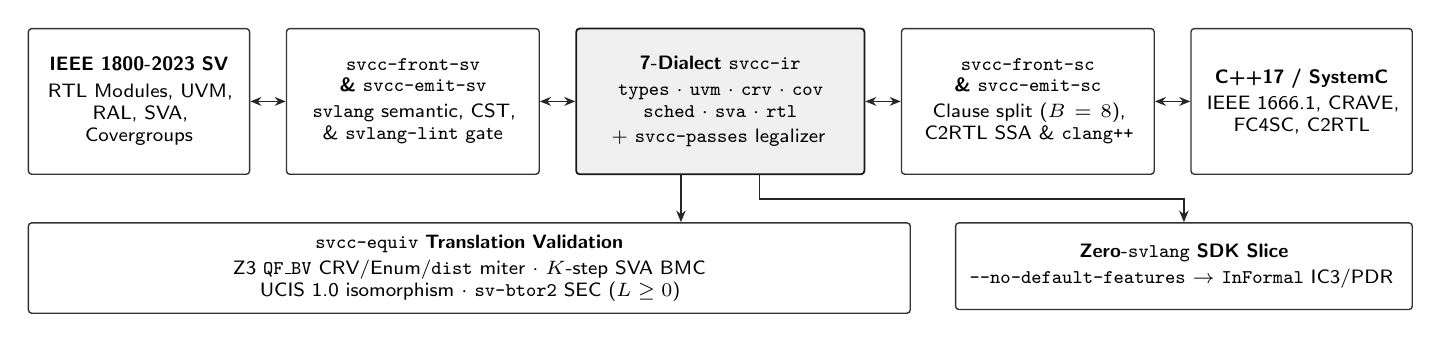
\begin{tikzpicture}[
  font=\sffamily\scriptsize,
  node distance=4.5mm,
  box/.style={
    draw=black!80,
    line width=0.5pt,
    rounded corners=1.2pt,
    fill=white,
    inner xsep=1.8mm,
    inner ysep=1.6mm,
    minimum height=18.5mm,
    align=center
  },
  irbox/.style={
    draw=black!90,
    line width=0.65pt,
    rounded corners=1.2pt,
    fill=black!6,
    inner xsep=1.8mm,
    inner ysep=1.6mm,
    minimum height=18.5mm,
    align=center
  },
  botbox/.style={
    draw=black!80,
    line width=0.5pt,
    rounded corners=1.2pt,
    fill=white,
    inner xsep=2.0mm,
    inner ysep=1.5mm,
    minimum height=11.0mm,
    align=center
  },
  arr/.style={-{Stealth[length=4.2pt,width=3.4pt]}, draw=black!85, line width=0.55pt},
  darr/.style={{Stealth[length=4.0pt,width=3.2pt]}-{Stealth[length=4.0pt,width=3.2pt]}, draw=black!85, line width=0.55pt}
]
  % Top row: 5 aligned pipeline stages (exact outer width = 175.0 mm)
  \node[box, text width=24.5mm] (svsrc) {%
    \textbf{IEEE 1800-2023 SV}\\[1.5pt]
    RTL Modules, UVM,\\
    RAL, SVA, Covergroups%
  };

  \node[box, text width=28.5mm, right=of svsrc] (svfe) {%
    \textbf{\code{svcc-front-sv}}\\[-0.5pt]
    \textbf{\& \code{svcc-emit-sv}}\\[1.5pt]
    \code{svlang} semantic, CST,\\
    \& \code{svlang-lint} gate%
  };

  \node[irbox, text width=33.0mm, right=of svfe] (svccir) {%
    \textbf{7-Dialect \code{svcc-ir}}\\[1.5pt]
    \code{types} $\cdot$ \code{uvm} $\cdot$ \code{crv} $\cdot$ \code{cov}\\
    \code{sched} $\cdot$ \code{sva} $\cdot$ \code{rtl}\\[1pt]
    + \textbf{\code{svcc-passes}} legalizer%
  };

  \node[box, text width=28.5mm, right=of svccir] (scfe) {%
    \textbf{\code{svcc-front-sc}}\\[-0.5pt]
    \textbf{\& \code{svcc-emit-sc}}\\[1.5pt]
    Clause split ($B=8$),\\
    C2RTL SSA \& \code{clang++}%
  };

  \node[box, text width=24.5mm, right=of scfe] (scsrc) {%
    \textbf{C++17 / SystemC}\\[1.5pt]
    IEEE 1666.1, CRAVE,\\
    FC4SC, C2RTL%
  };

  % Bottom row: exact outer span [svsrc.west .. scsrc.east] = 112.0 + 5.0 + 58.0 = 175.0 mm
  \node[botbox, text width=108.0mm, anchor=north west] (equiv)
    at ([yshift=-6.0mm]svsrc.south west) {%
    \textbf{\code{svcc-equiv} Translation Validation}\\[1.5pt]
    Z3 \code{QF\_BV} CRV/Enum/\code{dist} miter $\cdot$ $K$-step SVA BMC\\
    UCIS~1.0 isomorphism $\cdot$ \code{sv-btor2} SEC \mbox{($L \ge 0$)}%
  };

  \node[botbox, text width=54.0mm, anchor=north east] (sdk)
    at ([yshift=-6.0mm]scsrc.south east) {%
    \textbf{Zero-\code{svlang} SDK Slice}\\[1.5pt]
    \code{-{}-no-default-features} $\rightarrow$ \code{InFormal} IC3/PDR%
  };

  % Horizontal bidirectional compilation arrows
  \draw[darr] (svsrc.east) -- (svfe.west);
  \draw[darr] (svfe.east)  -- (svccir.west);
  \draw[darr] (svccir.east) -- (scfe.west);
  \draw[darr] (scfe.east)  -- (scsrc.west);

  % Orthogonal Manhattan routing from svcc-ir to bottom verification & SDK bars
  \coordinate (ir_l) at ([xshift=-5.0mm]svccir.south);
  \coordinate (ir_r) at ([xshift=5.0mm]svccir.south);
  \draw[arr] (ir_l) -- (ir_l |- equiv.north);
  \draw[arr] (ir_r) -- ++(0,-3.0mm) -| (sdk.north);
\end{tikzpicture}
\caption{The \code{svcc} compilation and translation-validation flow. Five core crates build with \code{-{}-no-default-features} without pulling in \code{svlang}, so external formal tools such as \code{InFormal} can link a pinned \code{svcc} commit cleanly.}
\label{fig:arch}
\end{figure*}

Figure~\ref{fig:arch} shows the \code{svcc} pipeline. The workspace contains 12,600 lines of Rust across eight Cargo crates (\code{svcc-ir}, \code{svcc-front-sv}, \code{svcc-front-sc}, \code{svcc-passes}, \code{svcc-emit-sc}, \code{svcc-emit-sv}, \code{svcc-equiv}, and the CLI/SDK crate \code{svcc}), plus a Python package (\code{svcc-py}, built with \code{PyO3} \code{abi3-py39}).

\subsection{Seven-Dialect svcc-ir and Capability Legalization}
An \code{IrModule} holds lowered design and testbench units in seven dialects:
\begin{itemize}
\item \textbf{\code{types}}: 2-state and 4-state packed vectors (\code{bit}, \code{logic}, \code{sc\_uint<W>}, \code{sc\_lv<W>}, \code{uint8\_t}--\code{uint64\_t}) and width-typed \code{EnumDecl} tables.
\item \textbf{\code{uvm}}: \code{ClassDecl} nodes tagged with \code{UvmRole} (\code{SequenceItem}, \code{Driver}, \code{Monitor}, \code{Scoreboard}, \code{Agent}, \code{Env}, \code{Reg}, \code{RegBlock}), RAL field slices (\code{lsb\_pos}, \code{access}, \code{volatile}, \code{reset}), address maps, TLM ports, and child components.
\item \textbf{\code{crv}}: A flat \code{CrvArena} indexed by 32-bit \code{ExprId} handles covering unary and binary bitvector math, implication (\code{->}), equivalence (\code{<->}), \code{inside} sets with \code{[c +/- d]} and \code{[c +\%- p]} tolerances, weighted \code{dist} (\code{:=} and \code{:/}), \code{unique} sets, and \code{soft} priorities.
\item \textbf{\code{cov}}: UCIS~1.0~\cite{accellera_ucis10} covergroups, coverpoints, value and range bins, ignore/illegal bins, and \code{cross} tables.
\item \textbf{\code{sched}}: Phase tasks (\code{run\_phase}), delays, event waits, \code{fork}/\code{join\_any}/\code{disable fork} groups, and \code{ClockingDecl} Preponed \code{\#1step} input skews.
\item \textbf{\code{sva}}: Concurrent \code{assert property} and \code{cover property} checks with clock edge, optional \code{disable iff} reset, antecedent, \code{\#\#[min:max]} delay window, and consequent.
\item \textbf{\code{rtl}}: Synthesizable \code{RtlModule} ports, internal wires, combinational logic (\code{always\_comb}, \code{SC\_METHOD}, \code{C2RTL} SSA cones), and sequential logic (\code{always\_ff}, \code{SC\_CTHREAD}).
\end{itemize}

Each target backend declares a \code{Target\allowbreak Capabilities} struct describing its memory model, process model, solver features, and assertion support. \code{PassPipeline::\allowbreak for\_target} runs four passes in order on \code{IrModule}: \code{Width\allowbreak Signedness\allowbreak Pass}, \code{FieldOp\allowbreak Synthesis\allowbreak Pass}, \code{Ownership\allowbreak Pass}, and \code{Target\allowbreak Legalizer\allowbreak Pass}.

\subsection{svlang Integration and Standalone CST Recovery}
Engineers and coding agents often translate one SystemVerilog file at a time (for example, \code{axi4\_burst\_env.sv} or \code{dma\_ch\_ral\_sva.sv}) without setting up a full simulator build list. When \code{uvm\_pkg} and companion package headers are missing, a purely semantic front end leaves UVM base classes unresolved and collapses parameterized ports such as \code{uvm\_analysis\_port \#(axi4\_item)} to error types. \code{svcc} builds on five Rust crates from \code{svlang}~\cite{kubavat2026svlang} to handle both full and partial context: \code{sv-semantic} for elaborated port widths and \code{TypeOracle} constant folding (\code{parameter}, \code{localparam}, \code{\$clog2}); \code{svlang-model} for UVM role classification; \code{sv-syntax} for lossless CST fallback that recovers \code{extends} names, \code{uvm\_reg}/\code{uvm\_reg\_block} roles, \code{`uvm\_field\_int} flags, and TLM port types directly from source tokens; \code{svlang-lint} to run \code{formal-ready} checks on emitted SystemVerilog; and \code{sv-netlist}/\code{sv-btor2} for word-level sequential miter generation. Passing \code{-{}-no-cst-fallback} turns off CST recovery for ablation testing.

\subsection{Clause Splitting, Solver Legalization, and SDK Slicing}
CRAVE represents each \code{crave::\allowbreak crv\_\allowbreak constraint} constructor as a nested Boost.Proto expression-template tree~\cite{haedicke2012crave,veldhuizen1995expr}. Generating C++17 text takes microseconds, but \code{clang++ -O2} spends superlinear time instantiating deeply nested templates as clause count $K$ grows. Because hard constraints are conjoined, \code{ScEmitter} offers \code{-{}-partition-clauses B}, splitting any block above $B$ clauses into \code{c\_\_part\_0}, \code{c\_\_part\_1}, and so on. On reverse \code{sc2sv} translation, \code{ScFrontend} merges \code{\_\_part\_} sub-blocks back into one SystemVerilog \code{constraint} block.

Live testing against CRAVE also exposed two solver corners that \code{svcc-passes} and \code{svcc-emit-sc} handle before code generation. First, when a hard bound such as \code{x >= 1} cuts across a \code{weighted\_range}, CRAVE clamps the excluded probability mass onto the boundary value instead of renormalizing. \code{Target\allowbreak Legalizer\allowbreak Pass} collects unsigned relational bounds from hard clauses, clips \code{dist} intervals to the feasible range, and scales \code{:/} weights by the $u128$ LCM of range denominators (leaving 32-bit spans whose scaled product exceeds \code{u32::MAX} to CRAVE's range sampler). Second, CRAVE rejects native \code{randc} variables wider than 16 bits and slows down sharply when cyclic exclusion lists are encoded as SMT clauses. \code{ScEmitter} therefore generates a 32-byte header-only 4-round cycle-walking Feistel permutation (\code{svcc\_randc\_feistel<W>}, $1 \le W \le 32$) that visits every value in $[0, 2^W - 1]$ once per period in $O(1)$ time.

To let formal tools such as \code{InFormal}~\cite{kubavat2026informal} embed \code{svcc}'s C2RTL lifter without clashing with \code{InFormal}'s own pinned \code{svlang} crates, \code{svcc-emit-sv} and \code{svcc-equiv} put \code{svlang} behind optional Cargo features (\code{verify-svlang} and \code{btor2-sec}). Compiling \code{svcc-ir}, \code{svcc-front-sc}, \code{svcc-passes}, \code{svcc-emit-sv}, and \code{svcc-equiv} with \code{-{}-no-default-features} produces a standalone C++-to-SystemVerilog miter library with zero \code{svlang} dependencies.

\section{Equivalence Checks and C-to-RTL Proof}
\label{sec:equiv}

Every \code{svcc} run can pass four automated checks before generated code is committed:
\begin{enumerate}
\item \textbf{Compiler and semantic lint gate.} Emitted C++17 headers must pass \code{clang++ -std=c++17 -Wall -Wextra -Werror} against open SystemC/UVM/CRAVE/FC4SC headers. Emitted SystemVerilog must elaborate cleanly in \code{svlang} and pass \code{svlang-lint}'s \code{formal-ready} rule set.
\item \textbf{\code{QF\_BV} constraint, enum, and \code{dist} miter.} For any pair of classes $(C_{\text{lhs}}, C_{\text{rhs}})$, \code{svcc-equiv} models each \code{rand}/\code{randc} field as an exact-width SMT-LIB2 bitvector \code{(\_ BitVec W)}, adds IEEE~1800 legal enum-variant constraints, encodes hard clauses and positive-weight \code{dist} support sets, and checks \code{(assert (xor c\_lhs c\_rhs))} in Z3~\cite{demoura2008z3}. \code{unsat} proves identical legal transactions across all $2^{\sum W_i}$ assignments; \code{sat} prints a concrete counterexample.
\item \textbf{Bounded model checking of SVA observers.} For each property with window \code{\#\#[m:n]}, \code{prove\_sva\_\allowbreak bmc\_\allowbreak equivalence} unrolls the IEEE~1800 assertion semantics and the generated 64-bit C++17 shift-window observer over $K = n + 6$ cycles under free \code{ant}, \code{con}, and \code{disable iff} inputs. For \code{cover property}, \code{prove\_sva\_\allowbreak cover\_\allowbreak multiplicity\_\allowbreak bmc} checks per-cycle hit increments between the \code{pending\_age\_} counter array and overlapping IEEE~1800 evaluation attempts.
\item \textbf{UCIS~1.0 bin isomorphism and Btor2 SEC.} Covergroups are checked for one-to-one coverpoints, bin intervals, and crosses. For RTL modules and untimed C++17 \code{// svcc:c2rtl} functions, \code{svcc-equiv} builds a miter module that drives both sides from shared inputs, delays the combinational C2RTL output through $L$ reset-initialized pipeline registers, lowers the miter through \code{svlang}'s netlist and \code{sv-btor2}~\cite{niemetz2018btor2,kubavat2026svlang}, and proves post-reset output agreement in Z3.
\end{enumerate}

\section{Evaluation}
\label{sec:eval}

I ran all experiments on one Apple silicon workstation (macOS arm64, Rust~1.93.0 \code{-{}-release}, Apple \code{clang++}~21.0.0, Z3~4.13, \code{svlang} commit \code{478a0d10}, and installed SystemC~3.0.3, UVM-SystemC, CRAVE, and FC4SC \code{development} libraries~\cite{kubavat2026scbench}). Two scripts (\code{benchmarks/run\_benchmarks.py} and \code{benchmarks/run\_m4\_extended.py}) regenerate the corpus, compile the live C++17 binaries, and write the JSON result files. The evaluation answers five questions:
\begin{itemize}
\item \textbf{RQ1 (Round-trip fidelity, C2RTL SEC, and speed):} Does \code{svcc} produce warning-free code and prove equivalence across UVM VIPs, RAL+SVA blocks, and pipelined RTL/C2RTL pairs at sub-millisecond compile speeds?
\item \textbf{RQ2 (Bug recall and equivalent-rewrite specificity):} Do the formal checks catch subtle bugs across CRV, SVA, UCIS, and RTL without flagging valid syntactic rewrites?
\item \textbf{RQ3 (Standalone VIP recovery):} How many single-file UVM/RAL inputs compile cleanly with CST fallback enabled versus strict semantic-only lowering?
\item \textbf{RQ4 (CRAVE C++17 compile time):} How much does \code{-{}-partition-clauses 8} reduce \code{clang++ -O2} compile time as constraint size $K$ grows?
\item \textbf{RQ5 (Live Accellera execution and external silicon code):} How do \code{svcc}'s \code{dist}, \code{cover property}, and Feistel \code{randc} lowerings behave under live CRAVE/FC4SC execution, and what happens on unmodified external SystemVerilog files?
\end{itemize}

\subsection{RQ1: 20-Design Benchmark Suite}

\begin{table*}[t]
\centering
\caption{RQ1 results on the 20-design suite (100-run mean compile time, \code{clang++ -Werror}, \code{svlang}/\code{svlang-lint}, Z3 round-trip proof time, and C2RTL sequential equivalence at pipeline latency $L$).}
\label{tab:rq1}
\footnotesize
\setlength{\tabcolsep}{3.1pt}
\begin{tabular}{@{}l l r r r r r r c c r c@{}}
\toprule
\textbf{Design} & \textbf{Category} & \textbf{LOC} & \textbf{Cls/RTL/SVA} & \textbf{CRV} & \textbf{\code{sv2sc} ($\mu$s)} & \textbf{\code{sc2sv} ($\mu$s)} & \textbf{RT Z3 (ms)} & \textbf{RT} & \textbf{$L$} & \textbf{SEC Z3 (ms)} & \textbf{SEC} \\
\midrule
\code{01\_apb4\_timer\_vip}    & UVM CRV VIP & 50 & 1 / 0 / 0 & 34 & 219 & 689 &  5.51 & \code{Unsat} & -- & --   & -- \\
\code{02\_axi4\_burst\_vip}    & UVM CRV VIP & 88 & 4 / 0 / 0 & 23 & 369 & 845 & 20.26 & \code{Unsat} & -- & --   & -- \\
\code{03\_pcie\_tlp\_hdr}      & UVM CRV VIP & 48 & 1 / 0 / 0 & 25 & 279 & 664 &  5.41 & \code{Unsat} & -- & --   & -- \\
\code{04\_chi\_coh\_req}       & UVM CRV VIP & 38 & 1 / 0 / 0 & 32 & 223 & 629 &  5.37 & \code{Unsat} & -- & --   & -- \\
\code{05\_eth\_mac\_frame}     & UVM CRV VIP & 41 & 1 / 0 / 0 & 29 & 190 & 631 &  5.42 & \code{Unsat} & -- & --   & -- \\
\code{06\_ddr5\_cmd\_sched}    & UVM CRV VIP & 59 & 2 / 0 / 0 & 21 & 265 & 719 & 10.35 & \code{Unsat} & -- & --   & -- \\
\midrule
\code{07\_uart\_16550\_ral}    & UVM RAL+SVA & 43 & 2 / 0 / 2 &  0 & 328 & 746 & 21.68 & \code{Unsat} & -- & --   & -- \\
\code{08\_dma\_ch\_ral\_sva}   & UVM RAL+SVA & 42 & 2 / 0 / 2 &  0 & 312 & 757 & 21.51 & \code{Unsat} & -- & --   & -- \\
\code{09\_spi\_master\_ral}    & UVM RAL+SVA & 41 & 2 / 0 / 1 &  0 & 324 & 688 & 14.84 & \code{Unsat} & -- & --   & -- \\
\code{10\_i2c\_ctrl\_ral\_sva} & UVM RAL+SVA & 39 & 2 / 0 / 2 &  0 & 291 & 755 & 21.14 & \code{Unsat} & -- & --   & -- \\
\code{11\_plic\_irq\_ral\_sva} & UVM RAL+SVA & 38 & 2 / 0 / 1 &  0 & 353 & 712 & 15.78 & \code{Unsat} & -- & --   & -- \\
\code{12\_wdog\_tmr\_ral\_sva} & UVM RAL+SVA & 38 & 2 / 0 / 1 &  0 & 302 & 766 & 16.24 & \code{Unsat} & -- & --   & -- \\
\midrule
\code{13\_alu32\_pipe2}        & RTL + C2RTL & 47 & 0 / 1 / 0 &  0 & 296 & 749 &  7.33 & \code{Unsat} & 2  & 7.29 & \code{Unsat} \\
\code{14\_mac16\_pipe2}        & RTL + C2RTL & 34 & 0 / 1 / 0 &  0 & 236 & 640 &  6.47 & \code{Unsat} & 2  & 6.34 & \code{Unsat} \\
\code{15\_crc8\_step\_comb}    & RTL + C2RTL & 18 & 0 / 1 / 0 &  0 & 162 & 576 &  6.85 & \code{Unsat} & 0  & 7.08 & \code{Unsat} \\
\code{16\_gray\_enc16\_pipe1}  & RTL + C2RTL & 20 & 0 / 1 / 0 &  0 & 156 & 532 &  6.02 & \code{Unsat} & 1  & 5.47 & \code{Unsat} \\
\code{17\_sat\_sub16\_pipe1}   & RTL + C2RTL & 25 & 0 / 1 / 0 &  0 & 168 & 554 &  5.87 & \code{Unsat} & 1  & 5.63 & \code{Unsat} \\
\code{18\_shifter32\_pipe2}    & RTL + C2RTL & 41 & 0 / 1 / 0 &  0 & 294 & 763 &  6.96 & \code{Unsat} & 2  & 5.95 & \code{Unsat} \\
\code{19\_minmax32\_pipe1}     & RTL + C2RTL & 31 & 0 / 1 / 0 &  0 & 184 & 605 &  5.81 & \code{Unsat} & 1  & 5.46 & \code{Unsat} \\
\code{20\_arb\_prio4\_comb}    & RTL + C2RTL & 22 & 0 / 1 / 0 &  0 & 154 & 576 &  6.86 & \code{Unsat} & 0  & 6.77 & \code{Unsat} \\
\midrule
\textbf{Total / Median}        & \textbf{20 designs} & \textbf{803} & \textbf{22 / 8 / 9} & \textbf{164} & \textbf{272} & \textbf{689} & \textbf{6.91} & \textbf{20/20} & \textbf{0--2} & \textbf{6.14} & \textbf{8/8} \\
\bottomrule
\end{tabular}
\end{table*}

Table~\ref{tab:rq1} shows results across the 20-design suite (28 files, 803 lines of SystemVerilog plus 8 untimed C++17 golden models). The suite covers six protocol VIPs (APB4, AXI4, PCIe TLP, Arm CHI, Ethernet MAC, and DDR5 DFI with \code{\#1step} clocking and \code{fork}/\code{join\_any}/\code{disable fork}), six peripheral RAL register blocks with concurrent SVA checkers (UART~16550, DMA, SPI, I2C, RISC-V PLIC, Watchdog), and eight synthesizable datapaths ($L \in \{0, 1, 2\}$ stages: 32-bit ALU, 16$\times$16+32 MAC, CRC-8 step, Gray encoder, saturating subtractor, barrel shifter, min/max unit, and priority arbiter) paired with untimed C++17 functions.

All 20 designs pass \code{clang++ -std=c++17 -Wall -Wextra -Werror -fsyntax-only} after \code{sv2sc}, pass \code{svlang} elaboration and \code{svlang-lint} \code{formal-ready} checks after \code{sc2sv}, and prove \code{EquivalentUnsat} across all 22 UVM classes, 9 SVA properties, and 8 RTL modules. Over 100 warm runs per file, \code{sv2sc} takes 154--369~$\mu$s (median 272~$\mu$s) and \code{sc2sv} (including \code{svlang-lint}) takes 532--845~$\mu$s (median 689~$\mu$s). Z3 round-trip proofs finish in 5.37--21.68~ms (median 6.91~ms, 215.7~ms total), and all 8 untimed C++17 reference functions prove equivalent to their pipelined RTL modules in 5.46--7.29~ms (median 6.14~ms).

\subsection{RQ2: Defect Mutations and Equivalent Rewrites}

\begin{table}[t]
\centering
\caption{RQ2 results on 20 injected bugs and 4 AST-different equivalent rewrites.}
\label{tab:rq2}
\footnotesize
\setlength{\tabcolsep}{3.5pt}
\begin{tabularx}{\columnwidth}{@{}l r r >{\raggedright\arraybackslash}X@{}}
\toprule
\textbf{Group} & \textbf{N} & \textbf{Result} & \textbf{Examples} \\
\midrule
CRV \code{QF\_BV}   & 8  & 8/8 \code{Sat}  & Align mask \code{3} to \code{1}, bound \code{0FFF} to \code{0FFB}, tol.\ halved, imp.\ flipped, \code{unique} dropped. \\
SVA \& UCIS         & 3  & 3/3 Caught      & Window \code{\#\#[1:4]} to \code{\#\#[1:3]}, \code{\#\#[1:3]} to \code{\#\#[2:3]}, MTU bin \code{46} to \code{64}. \\
RTL / C2RTL         & 9  & 9/9 \code{Sat}  & ALU XOR to OR, MAC addend drop, wrong latency $L=1$ vs.\ $2$, CRC poly \code{8C} to \code{8D}, prio.\ flip. \\
\midrule
Equiv.\ rewrites    & 4  & 4/4 \code{Unsat} & \code{0FFF} to \code{0FFE} under \code{(paddr\&3)==0}; \code{[c+/-10]} expanded; \code{x>=y} vs.\ \code{x>y} at \code{0} floor; XOR commute. \\
\bottomrule
\end{tabularx}
\end{table}

To check that \code{svcc-equiv} separates real semantic bugs from harmless syntax differences, I ran 20 non-equivalent mutations (\code{M01}--\code{M20}) and 4 equivalent rewrites (\code{E01}--\code{E04}), listed in Table~\ref{tab:rq2}. \code{svcc-equiv} flags all 20 bugs via \code{CounterexampleSat} or UCIS mismatch, including checking a 2-stage ALU at $L=1$ (\code{M14}) and shrinking an SVA window by one cycle (\code{M10}, \code{M11}). It also proves \code{EquivalentUnsat} with 0 false alarms on all 4 equivalent rewrites where AST diffing fails. For example, tightening an upper address bound from \code{32'h4000\_0FFF} to \code{32'h4000\_0FFE} (\code{E01}) leaves the legal register set unchanged because \code{(paddr \& 32'h3) == 32'h0} already caps aligned addresses at \code{32'h4000\_0FFC}, and changing \code{x >= y} to \code{x > y} in \code{sat\_sub16\_pipe1} (\code{E03}) gives the same result because $x - y = 0$ when $x = y$.

\subsection{RQ3 and RQ4: Standalone VIPs and Clause Splitting}

\begin{table}[t]
\centering
\caption{RQ3 standalone VIP recovery ($N=12$ files without \code{uvm\_pkg}) and RQ4 \code{clang++ -O2} compile time across $K$ CRAVE clauses.}
\label{tab:rq34}
\footnotesize
\setlength{\tabcolsep}{4pt}
\begin{tabularx}{\columnwidth}{@{}>{\raggedright\arraybackslash}X r r r@{}}
\toprule
\multicolumn{4}{@{}l}{\textbf{RQ3 (Prediction P6): Standalone UVM/RAL Files ($N=12$)}} \\
\midrule
\textbf{Frontend Mode} & \textbf{Role} & \textbf{\code{clang++}} & \textbf{Rate} \\
\midrule
Semantic-only (\code{-{}-no-cst-fallback}) & 4/12  & 4/12  & 33.3\% \\
Hybrid \code{svlang} + CST (default)     & 12/12 & 12/12 & \textbf{100.0\%} \\
\midrule
\multicolumn{4}{@{}l}{\textbf{RQ4 (Prediction P1): \code{clang++ -O2} Compile Time}} \\
\midrule
\textbf{Clauses ($K$)} & \textbf{Mono (ms)} & \textbf{Part-8 (ms)} & \textbf{Speedup} \\
\midrule
$K = 8$   &   245.9 & 246.2 & $1.00\times$ \\
$K = 24$  &   290.5 & 255.7 & $1.14\times$ \\
$K = 48$  &   394.3 & 261.5 & $1.51\times$ \\
$K = 80$  &   780.7 & 291.8 & $2.68\times$ \\
$K = 120$ & 1,845.4 & 295.1 & \textbf{$6.25\times$} \\
\bottomrule
\end{tabularx}
\end{table}

Table~\ref{tab:rq34} covers the two compiler ablations. In RQ3, translating the 12 UVM and RAL files without \code{-f} package lists succeeds on only 4 of 12 single-item files under \code{-{}-no-cst-fallback}, because missing \code{uvm\_reg}/\code{uvm\_reg\_block} base classes and parameterized TLM ports break the 8 multi-component and RAL files. Default hybrid \code{svlang}+CST mode recovers all 12 files (100\%, a $3.0\times$ gain).

In RQ4, I sweep clause count $K \in \{8, 24, 48, 80, 120\}$ under \code{clang++} \code{-std=c++17} \code{-O2} \code{-c}. A single monolithic \code{crv\_constraint} constructor grows from 245.9~ms at $K=8$ to 1,845.4~ms at $K=120$. Splitting at $B=8$ clauses per constructor (\code{-{}-partition-clauses 8}) holds compile time to 295.1~ms at $K=120$ ($6.25\times$ faster) while keeping Z3 \code{QF\_BV} equivalence and clean \code{sc2sv} re-merging.

\subsection{RQ5: Live Accellera Runs and External Silicon Code}

\begin{table*}[t]
\centering
\caption{RQ5 live SystemC 3.0.3 / UVM-SystemC / CRAVE / FC4SC measurements (\code{P2}, \code{P3}, \code{P5}) and 12-file unmodified external audit.}
\label{tab:m4}
\footnotesize
\begin{tabularx}{\textwidth}{@{}>{\raggedright\arraybackslash}p{1.25in} >{\raggedright\arraybackslash}X >{\raggedright\arraybackslash}p{2.30in}@{}}
\toprule
\textbf{Check} & \textbf{Setup and Baseline vs.\ \code{svcc} Lowering} & \textbf{Result} \\
\midrule
Live UVM + FC4SC     & Live binary: 200 UVM \code{randomize()} draws + \code{soft} override + \code{crv\_object\_name} stack fix & 100.0\% FC4SC coverage, 0 runtime/ASan errors \\
\midrule
\code{P2} \code{dist} ($10^5$ draws) & \code{[0:15] :/ 5, 16 := 5}: integer-floor per-element vs.\ $u128$ LCM \code{weighted\_range} & TVD $0.5000 \rightarrow \mathbf{0.0043}$ ($\chi^2$: $10^5 \rightarrow \mathbf{20.1}$) \\
\code{P2} \code{dist} ($10^5$ draws) & \code{[0:2] :/ 10, 3 := 2}: unscaled \code{weighted\_range} vs.\ $u128$ LCM \code{weighted\_range} & TVD $0.0055 \rightarrow \mathbf{0.0020}$ ($\chi^2$: $14.52 \rightarrow \mathbf{2.28}$) \\
\code{P2} sliced \code{dist}        & Hard bound (\code{x >= 1}, \code{x >= 8}): raw CRAVE clamping vs.\ \code{svcc} range clip + LCM & TVD $0.0978 \rightarrow \mathbf{0.0016}$ ($\chi^2$: $4541.6 \rightarrow \mathbf{1.64}$) \\
\midrule
\code{P3} \code{cover property}     & \code{\#\#[1:3]}--\code{\#\#[4:32]} overlapping bursts: 64-bit bitmask vs.\ per-age \code{pending\_age\_} & Removes $3\times$--$26\times$ burst \& $2.08\times$--$6.13\times$ $10^7$-cyc loss \\
\code{P3} Z3 BMC + speed            & Per-cycle increment miter ($n \le 32$) + $10^7$-cycle \code{clang++ -O2} throughput & \textbf{\code{EquivalentUnsat}} (32~ms Z3), \textbf{1.42--3.92~ns/cycle} \\
\midrule
\code{P5} \code{randc} ($W=10$)     & Live CRAVE history exclusion vs.\ \code{svcc\_randc\_feistel<10>} + Z3 follower constraint & $25.78\text{ ms/call} \rightarrow \mathbf{75.5~\mu\text{s/call}}$ ($\mathbf{341\times}$ faster) \\
\code{P5} \code{randc} ($W \ge 17$) & Native CRAVE \code{randc} (throws $>16$ bits) vs.\ \code{svcc\_randc\_feistel<W>} ($W \le 32$) & Runtime exception vs.\ \textbf{2.9--3.1~ns/call} (bijective) \\
\midrule
RQ5 External Files                  & 12 unmodified files (1,515 SV LOC: OpenTitan, PULP, OpenHW, Ibex, \code{InFormal}) & \textbf{9/12} (75\%) lowered standalone; \textbf{2/2} self-contained pass \code{-Werror} \\
\bottomrule
\end{tabularx}
\end{table*}

Header shims check C++ types, not solver behavior at run time. I therefore linked and ran \code{svcc}'s C++17 output against installed SystemC~3.0.3, UVM-SystemC, CRAVE (Z3 backend), and FC4SC libraries~\cite{accellera2026systemc,kubavat2026scbench} (Table~\ref{tab:m4}). A 200-transaction UVM testbench verified \code{soft} constraint overrides and closed 100.0\% FC4SC coverage with zero sanitizer or runtime errors.

Over $10^5$ live CRAVE draws per setup (\code{P2}), naive integer-floor \code{:/} division drops \code{[0:15] :/ 5} to zero weight (total variation distance $\text{TVD} = 0.500$, $\chi^2 = 10^5$), while \code{svcc}'s LCM scaling brings $\text{TVD}$ down to $0.0043$ and cuts $\chi^2$ on \code{[0:2] :/ 10, 3 := 2} from 14.52 to 2.28. When a hard constraint (\code{x >= 1} or \code{x >= 8}) cuts inside a \code{weighted\_range}, raw CRAVE piles excluded weight onto the boundary ($\text{TVD} = 0.0978$, $\chi^2 = 4541.6$). Clipping the range to hard bounds before LCM scaling drops $\text{TVD}$ to $0.0016$ ($\chi^2 = 1.64$, a $60.8\times$ reduction) and $0.0014$ ($\chi^2 = 2.54$). On \code{cover property} windows (\code{P3}), a 64-bit bitmask under-counts back-to-back bursts by $3\times$--$26\times$ and $10^7$ random cycles by $2.08\times$--$6.13\times$. \code{pending\_age\_} proves \code{EquivalentUnsat} in 32~ms of Z3 time and runs at 1.42--3.92~ns/cycle. On live \code{randc} sweeps (\code{P5}), CRAVE exclusion lists take 25.78~ms/call mean (26.40~s per 1,024-step cycle) at $W=10$, and native CRAVE \code{randc} throws an exception at $W \ge 17$. \code{svcc\_\allowbreak randc\_\allowbreak feistel<W>} runs in 2.9--3.1~ns/call standalone and 75.5--127.1~$\mu$s/call when coupled with Z3 follower constraints ($341\times$ faster at $W=10$, hitting all 65,536 values at $W=16$).

Finally, I ran \code{svcc sv2sc} without \code{-f} filelists on 12 unmodified external SystemVerilog files (1,515~LOC) from OpenTitan (\code{prim\_\allowbreak secded\_\allowbreak inv\_\allowbreak 39\_32\_dec.sv}, \code{prim\_\allowbreak fifo\_\allowbreak sync.sv}, \code{prim\_\allowbreak arbiter\_\allowbreak ppc.sv}), PULP \code{common\_\allowbreak cells}, OpenHW \code{core-v-verif}, lowRISC \code{ibex}, \code{InFormal}, \code{systemc-\allowbreak examples}, and \code{dv-\allowbreak patterns}. Nine of the 12 files (75.0\%) lower cleanly standalone. Both self-contained OpenTitan RTL blocks pass \code{clang++ -Werror} out of the box, and the remaining files fail closed with line-accurate messages on unexpanded vendor macros (\code{`FFARNC}), external \code{*\_pkg.sv} typedefs, or unpacked port arrays.

\section{Related Work}
\label{sec:related}

\textbf{SystemVerilog front ends and hardware IRs.} Open SystemVerilog front ends include Surelog/UHDM~\cite{dargelas2024surelog} and pure-Rust \code{svlang}~\cite{kubavat2026svlang}. Yosys~\cite{wolf2013yosys}, LLHD~\cite{schuiki2020llhd}, and MLIR/CIRCT~\cite{lattner2021mlir,circt2024} lower RTL for synthesis and simulation, while Verilator~\cite{snyder2020verilator} compiles RTL to C++ and SystemC cycle models. Built on \code{svlang}'s CST, semantic \code{TypeOracle}, UVM model, \code{svlang-lint}, and Btor2 crates, \code{svcc} adds bidirectional translation across UVM testbench classes, CRAVE constraints, FC4SC covergroups, SVA checkers, and synthesizable RTL.

\textbf{Translation validation and C-to-RTL equivalence.} Pnueli et al.~\cite{pnueli1998tv} and Alive2~\cite{lopes2021alive2} check compiler passes per run with SMT solvers, and Koelbl et al.~\cite{koelbl2009c2rtl} describe word-level sequential equivalence between C/C++ models and RTL. \code{svcc} brings per-run translation validation to the SystemVerilog/SystemC boundary by combining \code{QF\_BV} constraint miters, bounded SVA failure and hit-count proofs, UCIS bin isomorphism, and Btor2~\cite{niemetz2018btor2} SEC, while exposing a zero-\code{svlang} Rust slice for unbounded IC3/PDR proofs in \code{InFormal}~\cite{kubavat2026informal}.

\section{Threats to Validity and Conclusion}
\label{sec:conclusion}

\emph{Corpus scale.} Twenty benchmark designs and 12 external files cover common UVM, RAL, SVA, and datapath patterns, but do not span full chip-level multi-agent environments. All scripts and per-file JSON outputs are released so larger suites can be measured directly. \emph{Synthesizable C++17 subset.} \code{C2RTL} and \code{SC\_MODULE} lifting enforce IEEE~1666.1~\cite{ieee1666_1_2016} fail-closed rules, refusing heap allocation, STL containers, recursion, and multi-\code{wait()} scheduling. \emph{Bounded sequential depth.} Built-in Btor2 SEC and SVA checks unroll a bounded post-reset horizon at user-given latency $L$; unbounded proofs delegate to \code{InFormal}~\cite{kubavat2026informal}. \emph{Relational \code{dist} and sparse \code{randc}.} Static interval clipping handles single-variable constant bounds on \code{dist}, whereas multi-variable bounds cutting inside a \code{weighted\_range} and cyclic variables restricted to sparse subsets still need solver-side support. \emph{Single-file external closure.} CST fallback recovers missing \code{uvm\_pkg} roles, while external VIPs that depend on project \code{*\_pkg.sv} typedefs, vendor flip-flop macros, or unpacked port arrays need multi-file \code{-f} compilation support, which is planned next.

\code{svcc} pairs fast SystemVerilog/SystemC compilation over \code{svcc-ir} with Z3 and Btor2 sign-off checks so engineers and coding agents can iterate in C++17 without losing IEEE~1800 equivalence.

\textbf{Artifacts.} The \code{svcc} Rust workspace, Python bindings, 20-design corpus, live CRAVE/FC4SC probe, external audit scripts, and JSON results are maintained at \url{https://github.com/mayurkubavat/svcc}.

\textbf{Use of AI.} AI coding tools assisted in writing parts of the Rust implementation, benchmark scripts, and manuscript draft under the author's direction and review. The author verified every compiler check, solver proof, measurement, and reference, and takes full responsibility for this work.

\IEEEtriggeratref{14}
\bibliographystyle{IEEEtran}
\bibliography{../refs}

\end{document}
